\documentclass[11pt,a4paper,titlepage,oneside]{report}
\usepackage{titling}
\usepackage{graphicx}
\usepackage{mathtools}
\usepackage{lmodern}
\usepackage{amsmath}
\usepackage{float}
\usepackage{subfig}
\usepackage{listings}
\usepackage[hidelinks]{hyperref}

%% Memoir layout setup

%% NOTE: You are strongly advised not to change any of them unless you
%% know what you are doing.  These settings strongly interact in the
%% final look of the document.

% Dependencies
\usepackage{bfhlogo}
\usepackage{etoolbox}% http://ctan.org/pkg/etoolbox

\makeatletter
%%begin novalidate
%% Titlepage adjustments
\pretitle{\vspace{0pt plus 0.7fill}\begin{center}\Huge}
\posttitle{\end{center}\par}
\preauthor{\par\begin{center}\let\and\\\Large}
\postauthor{\end{center}}
\predate{\par\begin{center}\Large}
\postdate{\end{center}}
%%end novalidate
\def\@advisors{}
\newcommand{\advisors}[1]{\def\@advisors{#1}}
\def\@department{}
\newcommand{\department}[1]{\def\@department{#1}}
\def\@thesistype{}
\newcommand{\thesistype}[1]{\def\@thesistype{#1}}

\renewcommand{\maketitlehooka}{\noindent\bfhlogo[2cm]}

\renewcommand{\maketitlehookb}{\vspace{1in}%
  \par\begin{center}\Large\sffamily\@thesistype\end{center}}

\renewcommand{\maketitlehookd}{%
  \vfill\par
  \begin{flushright}
    \sffamily
    \@advisors\par
    \@department, BFH
  \end{flushright}
}

% Fix the chapters (unnecessary space)
\patchcmd{\@makechapterhead}{\vspace*{50\p@}}{}{}{}% Removes space above \chapter head
\patchcmd{\@makeschapterhead}{\vspace*{50\p@}}{}{}{}% Removes space above \chapter* head

\makeatother

\setlength{\droptitle}{-48pt}


\setlength{\parindent}{0pt}

\title{ORB Slam Point Cloud generation on Apalis iMX8}
\author{Stefan Eichenberger}
\date{December 2018}
\advisors{Marcus Hudritsch}
\department{TSM CPVR Lab}

\lstset{
	basicstyle=\ttfamily\scriptsize
}

\begin{document}
\maketitle

\begin{abstract}
	For robotic navigation a map of the robots environment is often required. Because robots often are small in size and independent of power plugs, they have limited processing power. This work analyzes how well one specific SLAM system is suitable for an embedded processor and what kind of improvements would be possible.
\end{abstract}

\section*{Executive Summary}
Simultaneous Location and Mapping (SLAM) is an important topic in computer vision today. The possibilities for this technology are infinite. SLAM can be used for navigation, object recognition and augmented reality. Often this algorithms need a high performance graphics card or a high performance processor. For industrial and robotics purposes we have constraints in space, thermal and power consumption. This doesn't allow the usage of a high performance CPUs. This work analyzes one specific SLAM algorithm on how it performs on a modern embedded ARM CPU. The long term goal is to have a system available that generates a map and to use this map for further navigation.

\tableofcontents

\chapter{Introduction}
To find the position of a robot we can use different sensors. Navigation systems use IMUs, magneto meters, radio signals and for outdoor navigation GPS. Humans however, do a lot of navigation by eye. Embedded systems today have enough processing power to do complex calculations. Therefore a possibility to estimate the position of the robot can also be computer vision. One field in computer vision is SLAM where we try to create a map of the environment and estimate the pose of the camera based on camera images. In this project we analyze the performance of ORB SLAM \cite{orbslam} running on an iMX8QM as embedded system. We use a Stereo Camera to create a point cloud and use this point cloud to calculate the changes in pose and position. By using a Stereo Camera we are able to reconstruct a point cloud with a known scale. This allows us to create a 3D map with real world scale of the environment around the camera.

\section{Apalis iMX8QM}

This project is supported with embedded hardware by Toradex. Toradex is a system on module provider focusing on embedded ARM devices for industrial applications.  They are interested to see some new applications and demos running on the new Apalis iMX8QM. Therefore, we concluded to try to port a computer vision application like SLAM to this platform. One area where NXP, the manufacturer of the processor, tries to place the iMX8 is computer vision in industry and automation, that's why it should be a good fit for this type of application. NXP has launched different types of iMX8. Publicly available today is only the iMX8M which is performance wise placed between the iMX8 and the iMX8X. The Apalis iMX8 Quad Max used in this project is the processor with highest performance. It will be release in 2019. We were using an Alpha Silicon version of the processor that was provided by Toradex.

\subsection{Features}

The iMX8QM has the following features:
\begin{itemize}
  \item Two Cortex A72 high performance processors
  \item Four Cortex A53 low power processors
  \item Two Cotex M4 realtime processors 
  \item Two Vivante GC7000 GPUs each with 8 cores that can calculated vec4 in float32
  \item Industrial temperature range from -40°C to 85°C
\end{itemize}

The iMX8 is focusing on industrial applications. Therefore it doesn't use state of the art production processes. The iMX8 is produced in 28nm structure while Smartphone processors already use 7nm technology. However, this make the processor less prone to high temperatures. The Cortex A72 also delivers good performance modern Smartphones today use Cortex A73 processors which are only one generation ahead. The Vivante GPU is a low end GPU that can be compared to middle class Smartphone GPUs. The two Cortex M4 processors could be used for Realtime processing. However, we don't use them in this work.

\section{Goals}
The goals of this project can be described as:
\begin{itemize}
\item Porting ORB SLAM to the Apalis iMX8
\item Analyzing different possibilities to speed up the algorithm
\item Add an extension to create a denser cloud
\item Evaluate the results and start discussion about further work.
\end{itemize}

The main focus of this work is to figure out how we can use or implement a SLAM algorithm that later could be used to reconstruct the world around the camera in 3D. This 3D world or 3D point cloud could in a later step, that is not part of this work, used to plan paths around obstacles and to estimate the position of a camera in a known environment.

\section{Time Plan}

The project was planned to end on beginning of January. The concept phase started well. Unfortunately, standard ORB SLAM didn't perform very well for our purposes. First optimizations only improved the performance a little bit. However, we implemented a dense point cloud generator based on this implementation to figure out what challenges we have to fight there. The time plan of this project is shown in figure \ref{fig:timeplan}.
\begin{figure}[H]
	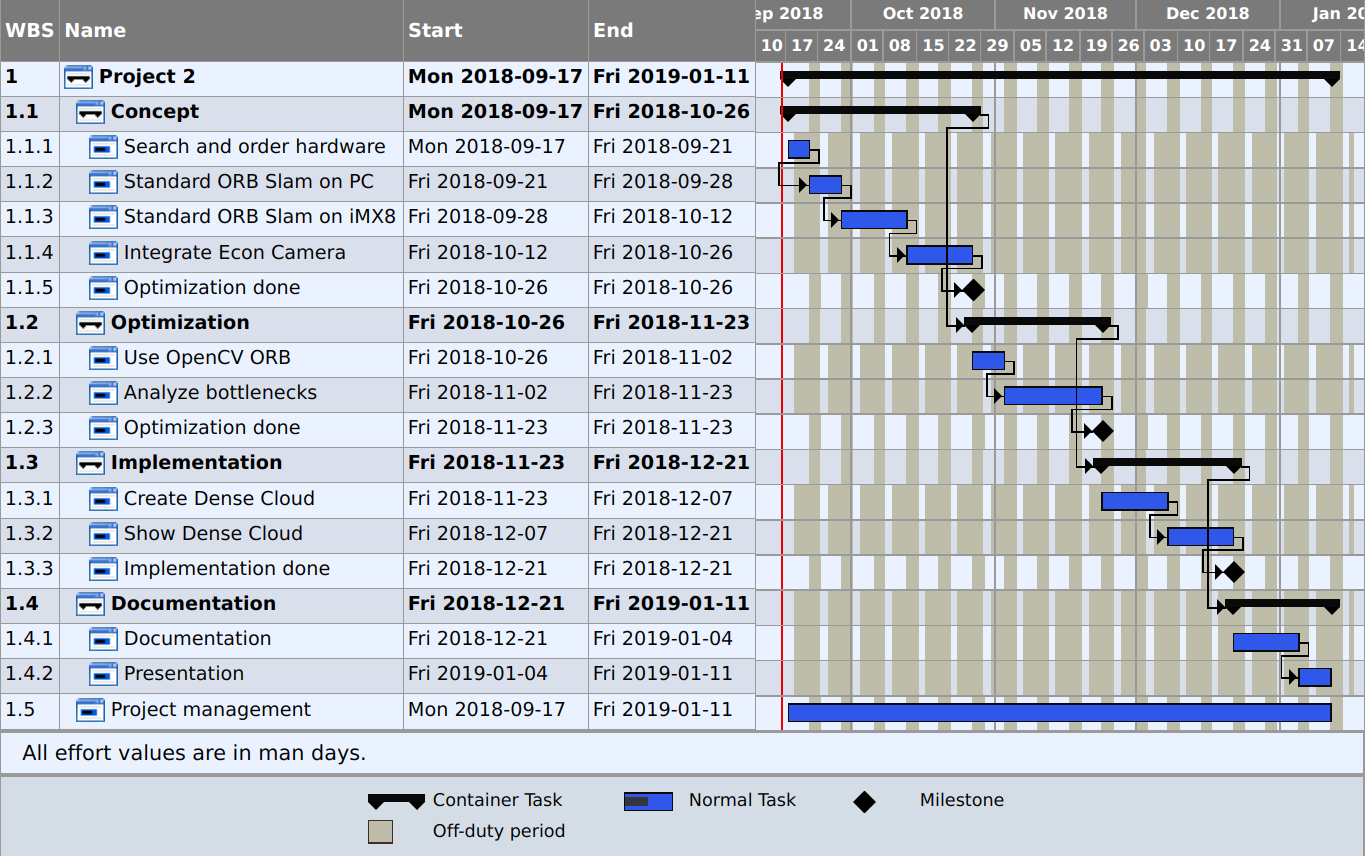
\includegraphics[width=1.0\textwidth]{img/timeplan.png}
	\caption{Time Plan}\label{fig:timeplan}
\end{figure}

\chapter{SLAM Evaluation}

In this section we analyze what kind of SLAM systems are already documented today. We can ruffly split them into two groups indirect and direct SLAM see figure \ref{fig:slammodes}.\\\\
Indirect methods analyze an image and try to extract features. This feature points are matched directly to further images. Based on this matches we can estimate the pose of the camera.
Direct methods on the other hand operated directly on intensity variances. The goal is to find a pose that minimizes the intensity difference between two images. Because minimizing the intensity difference over the whole image is computational expensive most methods operated only on edges or corners of the image. Such methods are called direct semi dense or direct sparse methods. In the next sections we will a have discussion about these different approaches.

\begin{figure}[H]
	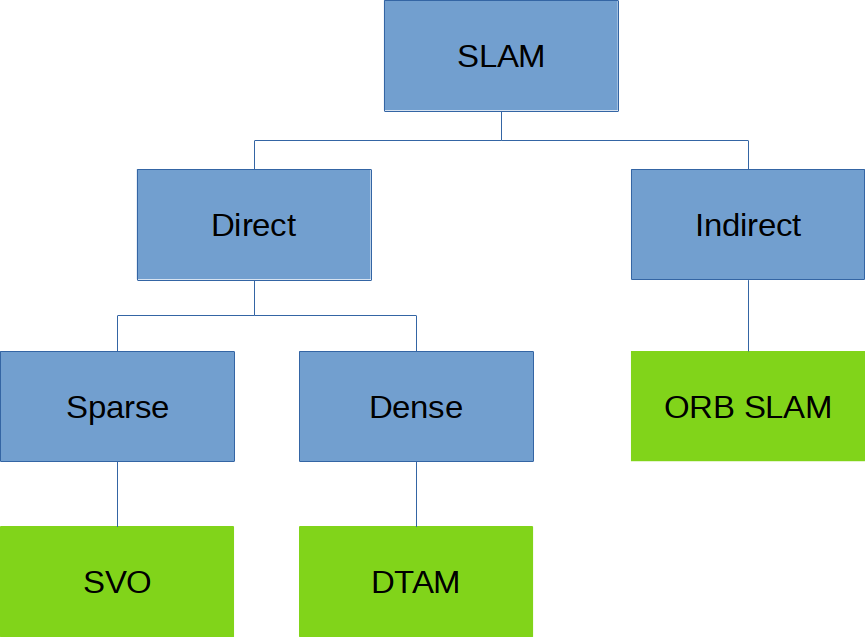
\includegraphics[width=1.0\textwidth]{img/slam_modes.png}
	\caption{SLAM Modes}\label{fig:slammodes}
\end{figure}


\section{Indirect method}

A well documented indirect method is ORB SLAM \cite{orbslam}. ORB SLAM extracts keypoints and calculates the ORB descriptors \cite{orb} around it. In further frames it again extracts ORB keypoints and matches them with the already known descriptors. Based on this matches it can do triangulation with RANSAC \cite{ransac} to estimate the current pose and position. Indirect methods have the advantage that the pose estimation can be done trough triangulation which isn't computational expensive. On the other side computing descriptors cost CPU time.

\section{Direct method}

In this section we will analyze two direct approaches a dense and a sparse approach. Dense methods use all pixels on the image for tracking while sparse methods only use a subset. Figure \ref{fig:sparse_dense} shows a comparison of dense sparse and semi-dense approaches. We don't dig into semi-dense approaches they work similar to sparse methods but with more keypoints.

\begin{figure}[H]
  \begin{center}
		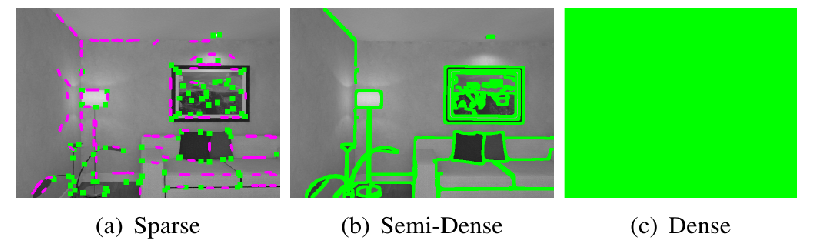
\includegraphics[width=1.0\textwidth]{img/sparse_dense.png}
  \end{center}
	\caption{Comparison of sparse, dense and semi-dense approaches from paper \cite{svo}}\label{fig:sparse_dense}
\end{figure}

\subsection{Dense}

There are not that many dense SLAMs. One is DTAM \cite{dtam} which uses the intensity values of the whole image to do the pose estimation. The idea is to minimize the intensity difference (energy) between two images by optimizing the camera pose. The energy defined at one pixel position is defined as shown in \ref{eq:pixel_energy}. To estimate the Pose it tries to find a P that minimizes $E_{t}$ as shown in \ref{eq:total_energy}.
\begin{equation}\label{eq:pixel_energy}
  E_{u}=I_1(u)-I_2(P*U)
\end{equation}
Where:
\begin{align*}
  E_{u}		&: \text{Energy at a specific position}\\
  I_{1/2}	&: \text{Image 1/2}\\
  u		&: \text{Position in image} \\
  P		&: \text{Pose of the camera} \\
  U		&: \text{Position of x in 3D}
\end{align*}
\begin{equation}\label{eq:total_energy}
  E_{t}=\min(\sum_{x=0}^X\sum_{y=0}^YE_u)
\end{equation}
Where:
\begin{align*}
  E_{t}		&: \text{Total energy}\\
  E_{u}		&: \text{Energy at a specific position}\\
	X				&: \text{Image columns}\\
	Y				&: \text{Image rows}\\
\end{align*}


One of the biggest advantages of using a direct dense method is that we receive a dense point cloud which can be used directly to create maps and 3d objects. A big disadvantage is however that they are quite computational expensive. Therefore they are not appropriate for embedded devices.

\subsection{Sparse}

Sparse direct SLAMs like SVO \cite{svo} don't optimize the Energy over the whole image but the energy at sparse points instead. One possibility of a sparse point is e.g. a corner point found by FAST \cite{fast}. Similar to sparse methods there are semi dense methods which try to minimize the energy with several points laying on edges. They can e.g. be found by Canny Edge detection or DoG. The advantage of sparse and semi dense are that such methods are less computational expensive than dense methods.\\\\

Sparse direct methods don't create dense clouds immediately however they are able to work on weaker keypoints than indirect methods. Therefore they can create denser clouds than e.g. ORB SLAM. They can also be computational less expensive than indirect methods because they don't have to calculate expensive features.

\section{Stereo and Monocular SLAM}

In this project the focus is on Stereo SLAM. A lot of todays paper focus on monocular SLAM. The reason that first Monocular cameras are cheaper and second Monocular cameras are available in Smartphones. Monocular SLAM has two main problems. First an initialization process needs to estimated the movement between two frames. A 3D point cloud can only be produced with two images with known position. In the monocular case the position of two images is random. Therefore the algorithm needs to guess the pose and transformation over a few images until it knows the pose. It does that by taking some assumption on the world or by trying to optimizing the point positions over several images. However, even when successfully initialize the second problem persists. In monocular SLAM we are not able to guess the scale of the point cloud. The intuition for this issue is that we can't distinguish between the movement of the camera on a small model close to the scene or the movement of the camera on the original model farer away from the scene. For stereo SLAM we don't have this issues. For each camera pose we get two images with known distance between the two camera sensors (baseline). Therefore, we can calculate the depth of each pixel in real world distance. From this we can generate a point cloud assuming that the initial camera pose starts at (0,0,0). We therefore have an instantaneous initialization and can calculate the real world position in a known unit e.g. meters. Tracking between two camera poses is however similar for monocular and stereo SLAM. For stereo SLAM tracking is often done only on one image. However keypoints can again be inserted immediately on stereo cameras without the need of using a second camera pose. This makes stereo SLAM more robust than monocular SLAM.

\section{Decision}

In this project we will port ORB SLAM onto iMX8 and see how it performs. We decided to use ORB SLAM because of the following criteria:
\begin{itemize}
	\item Open Source implementation available
	\item Powerful framework for displaying Point Cloud and images
	\item Good documentation
	\item Indirect methods seem promising because triangulation can be fast
	\item The CPVR lab already has experience with ORB on Smartphones
\end{itemize}

Based on ORB SLAM we try to analyze how we can use the iMX8 and whether ORB SLAM fits well for this target.

\chapter{Camera Evaluation}

To do stereo vision we need a stereo camera. There are a few stereo camera available on the market. It is also possible to build a stereo camera with two monocular cameras. However, we decided against that because it would require a mechanism to synchronize the images from both streams. We analyze three stereo cameras that are available on the market.

\section{ZED}
The ZED camera is a relatively new stereo camera from Stereo Labs. Here a feature list:
\begin{itemize}
	\item Full HD color images with 30fps
	\item USB3.0
	\item UVC compliant
	\item Linux SDK
	\item Baseline 120mm
	\item IMU sensor with 6DoF
	\item Price: 449\$
\end{itemize}

To run their SDK a Dual Core CPU with 2.3 GHz and CUDA > 3.0 is required. However, it's also possible to use the camera without their SDK.

\section{ECON Tara}
The Tara camera from Econ is another stereo camera. In comparison to the ZED camera it delivers a reduced resolution and only gray scale images.
\begin{itemize}
	\item 752x480 gray scale images with 60fps
	\item USB3.0
	\item Global Shutter Camera
	\item UVC compliant
	\item Baseline 60mm
	\item IMU sensor with 6DoF
	\item Open Source SDK
	\item Price: 149\$
\end{itemize}

It has a small OpenCV based SDK with open source software. In comparison to the ZED SDK it is less powerful.

\section{Intel RealSense D430}
The Intel RealSense camera is a infrared stereo camera. In comparison to RGB stereo camera it uses infrared images for stereo vision. It seems that this sensors are less prone for reflection. A third camera delivers RGB images in full HD.
\begin{itemize}
	\item 1280x720 with 90fps (IR), 1920x1080 with 30fps (RGB)
	\item USB3.0
	\item Global Shutter Camera
	\item UVC compilant (kernel patch required)
	\item Baseline 50mm
	\item Open Source SDK (librealsense)
	\item Price: 179\$
\end{itemize}

The Intel SDK seems quite powerful and is open source as well. However the indepth details of the camera are not publicly available.

\section{Decision}

Because the Econ Tara has an outstanding price ratio and because it is a conventional stereo camera we decide to use this camera. However, the Intel RealSense camera would be a great fit as well because it delivers a depth image directly. This would reduce the CPU load of the iMX8. If Full HD is required the ZED could also fit but keep in mind that for embedded systems Full HD processing may not be possible. We decided against this camera because of the high price and because of the closed source SDK.

\chapter{Camera Calibration}

Camera calibration is necessary to find a model that expresses the properties of a camera. Properties of a camera are:

\begin{itemize}
	\item Focal length of the camera lense
	\item Principal point on the camera sensor, where the z axis of the cameras coordinate system goes through.
	\item Distortion of the camera lense
	\item Size of a pixel
\end{itemize}

One example where we need to know the camera model is if we project virtual objects into a real world image. Figure \ref{fig:model} shows an image of a checkerboard where we project a virtual cube onto. One camera model in this image took distortion into account while the other one ignored it.
\begin{figure}[H]
  \begin{center}
		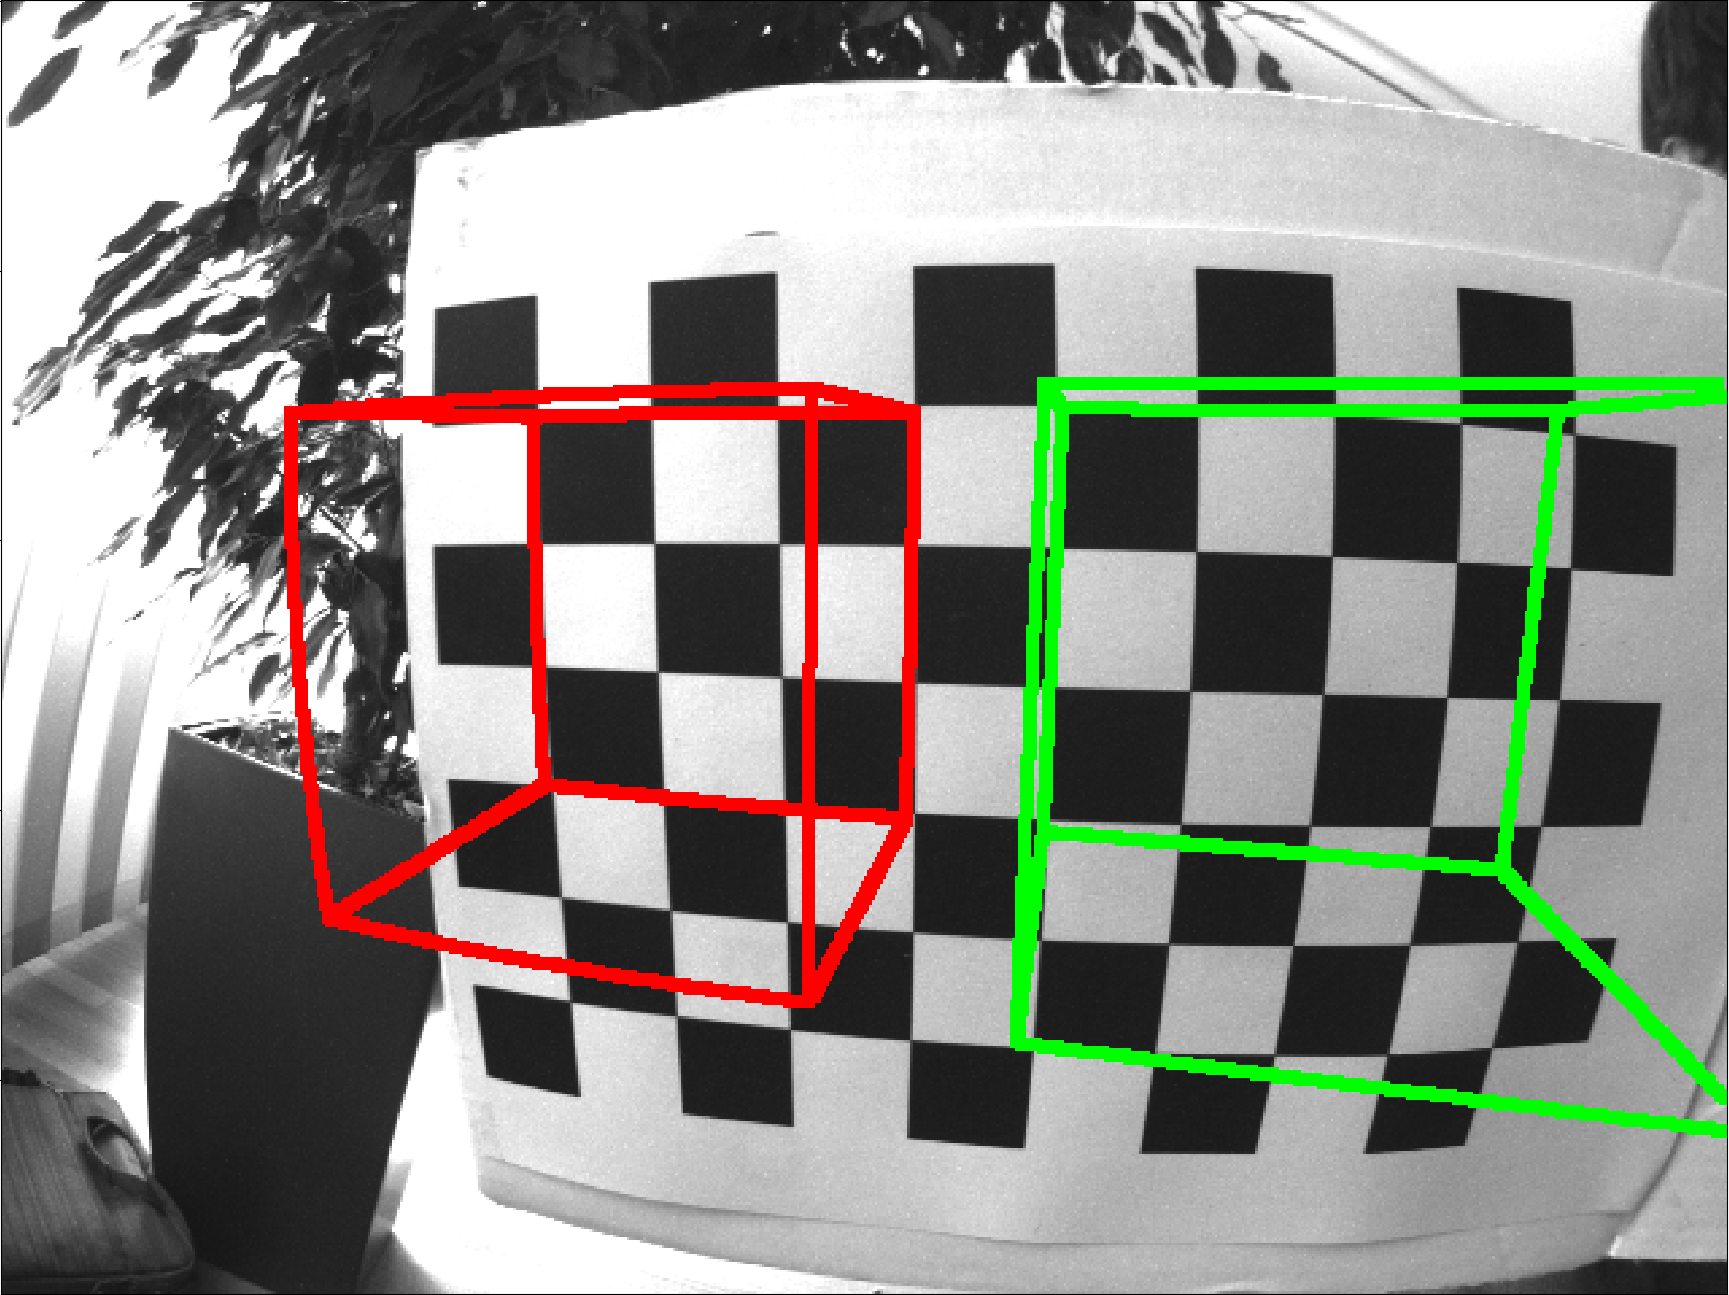
\includegraphics[width=1.0\textwidth]{img/model.png}
  \end{center}
	\caption{Applied camera model with (red) and without(green) distortion}\label{fig:model}
\end{figure}

We also need to know the camera model when doing SLAM. With known camera model we can rectify (see \ref{fig:calibration_real}) the image so that we can assume the camera as a ``perfect'' pinhole camera with known image center and known focal width.

Additional to the above parameters we need to align the images of the left and right camera in stereo vision. This process is called rectifying. The cameras aren't perfectly aligned in horizontal direction however we need to have them aligned because this makes it possible to search for correspondence only on the epipolar line. Further the cameras are slightly rotated which means we must inverse rotate the image to have a perfect alignment. So additional to the properties of the camera we need to know the following parameters:
\begin{itemize}
	\item Rotation matrix of the right camera in regards to the left
	\item Y offset of the right and left camera in pixels to align the images perfectly
\end{itemize}

\section{Camera Model}

The camera model expresses how any point in the three-dimensional space is projected onto a two-dimensional image. As a first approximation it assumes that all rays are going trough one point. This is called the pinhole camera model \ref{fig:projection}a. Given this assumption we can describe the projection of a 3D point onto a 2D image as shown in equation \ref{eq:cm}. We calculate the pixel location $x,y$ on the image by normalizing with $s$ as show in equation \ref{eq:cm_normalized} \cite{rvc}.
\begin{equation}\label{eq:cm}
  \begin{pmatrix}
		f_x & \gamma & c_x \\
		0 & f_y & c_y \\
		0 & 0 & 1 \\
	\end{pmatrix}*
	\begin{pmatrix}
		r_{00} & r_{01} & r_{02} & t_x \\
		r_{10} & r_{11} & r_{12} & t_y \\
		r_{20} & r_{21} & r_{22} & t_z \\
	\end{pmatrix}
	\begin{pmatrix}
		X \\
		Y \\
		Z \\
		1
	\end{pmatrix}=
	\begin{pmatrix}
		u \\
		v \\
		s
  \end{pmatrix}
\end{equation}
\begin{equation}\label{eq:cm_normalized}
	\begin{pmatrix}
		x \\
		y
	\end{pmatrix}=
	\begin{pmatrix}
		u/s \\
		v/s 
  \end{pmatrix}
\end{equation}

Where:
\begin{align*}
  X,Y,Z			&: \text{point in the 3D world}\\
	u,v,s	   	&: \text{point in 2D image not normalize}\\
	x,y				&: \text{point in 2D image normalized with s}\\
	f_x,f_y  	&: \text{focal length of the camera}\\
  c_x,c_y  	&: \text{principal point}\\
  t_x,t_y,t_z	&: \text{location of the camera}\\
  r_{ij}	&: \text{part of the rotation matrix}
\end{align*}

We can describe the intuition as follows. A Point (X,Y,Z) is projected onto an image sensor (u/s,v/s) by the multiplication of the intrinsic times the extrinsic matrix. The extrinsic matrix describes where the pinhole of the camera is located in the three dimensional space. The intrinsic camera matrix describes how the camera is constructed. For example, in figure \ref{fig:projection}b we translate and rotate a point $p_i$ with the extrinsic matrix so we can describe its coordinates with the pinhole as origin. Further we transform the point with the intrinsic camera matrix onto the image sensor.

\begin{figure}[H]
	\centering
	\subfloat[Pinhole model]{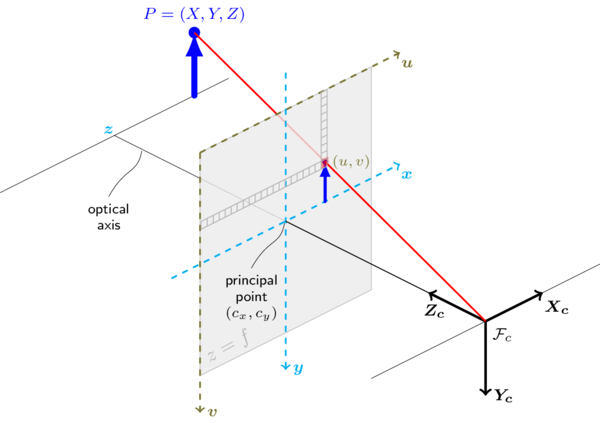
\includegraphics[width=0.5\textwidth]{img/pinhole_camera_model.png}}
	\subfloat[3D point to 2D point]{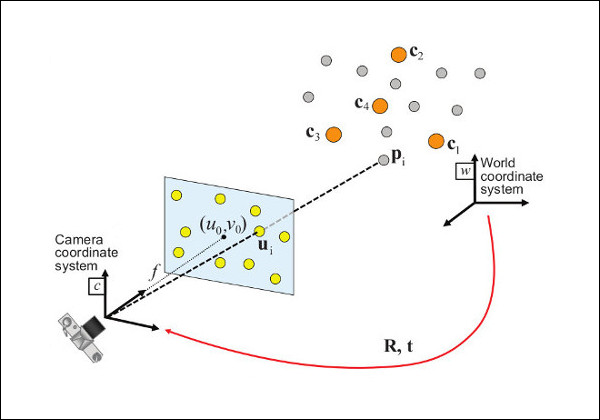
\includegraphics[width=0.5\textwidth]{img/pnp.jpg}}
	\caption{Image projection}\label{fig:projection}
\end{figure}

In SLAM if we know the intrinsic camera matrix we can calculate the pose by multiplying the projection matrix with the inverse of the intrinsic matrix.

\section{Stereo Camera Model}

Additional to the monocular parameters we need to find the parameters of the stereo camera. An image taken by a stereo camera normally is misaligned as shown in the top row of figure \ref{fig:stereo_calib}. The goal is to find the rotation matrix as well as the Y offset to get a perfectly aligned image pair as shown in the bottom row of figure \ref{fig:stereo_calib}.

\begin{figure}[H]
  \begin{center}
		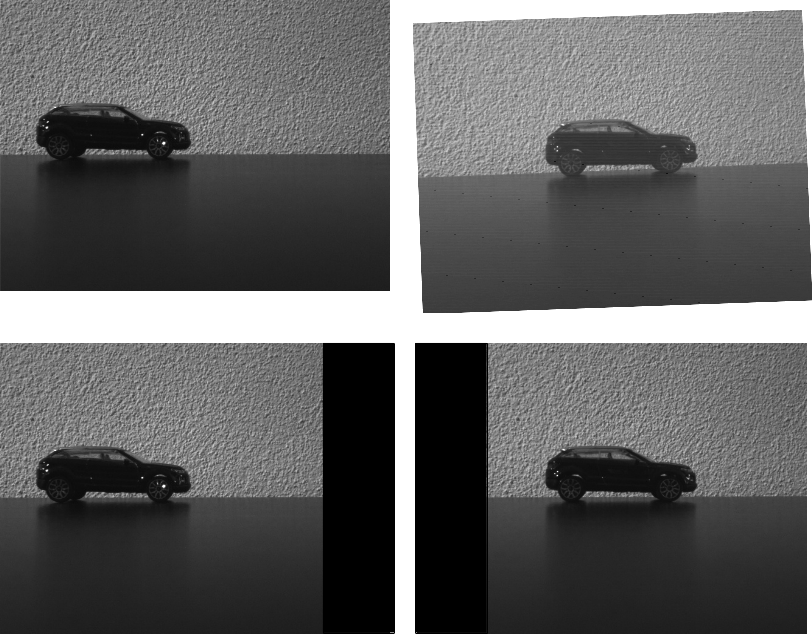
\includegraphics[width=0.9\textwidth]{img/stereo_calib.png}
  \end{center}
	\caption{Stereo Calibration, top row misaligned image, bottom row rectified images}\label{fig:stereo_calib}
\end{figure}

\begin{figure}[H]
	\centering
	\subfloat[left image used for calibration]{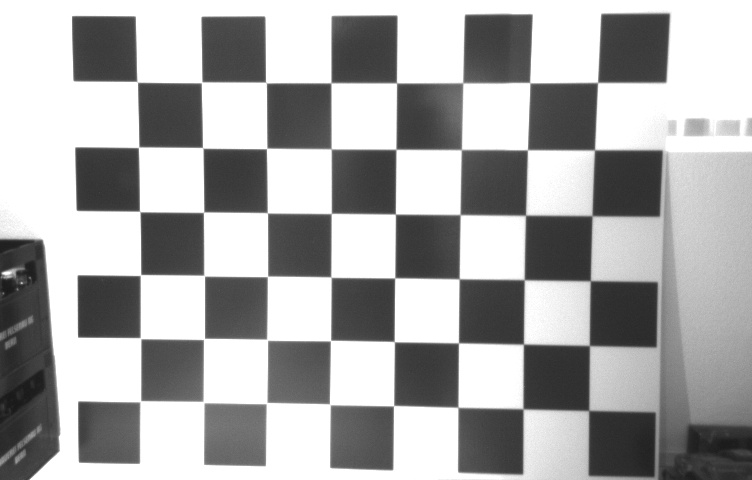
\includegraphics[width=0.4\textwidth]{img/calib0_left.jpg}}
	\subfloat[right image used for calibration]{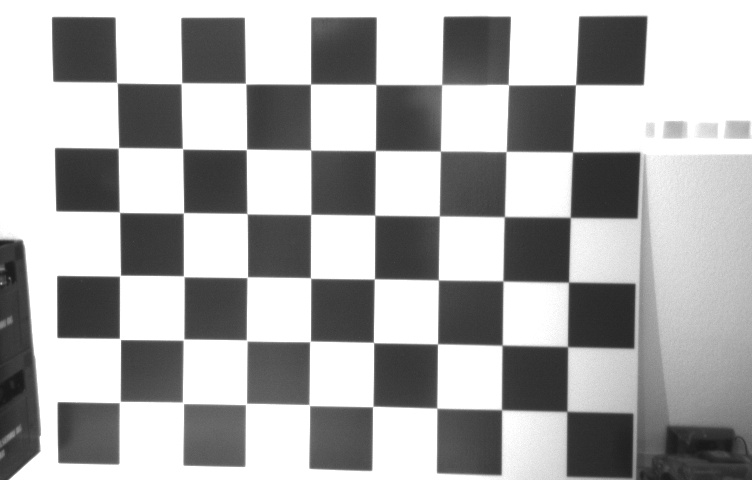
\includegraphics[width=0.4\textwidth]{img/calib0_right.jpg}}\\
	\subfloat[left image after rectification]{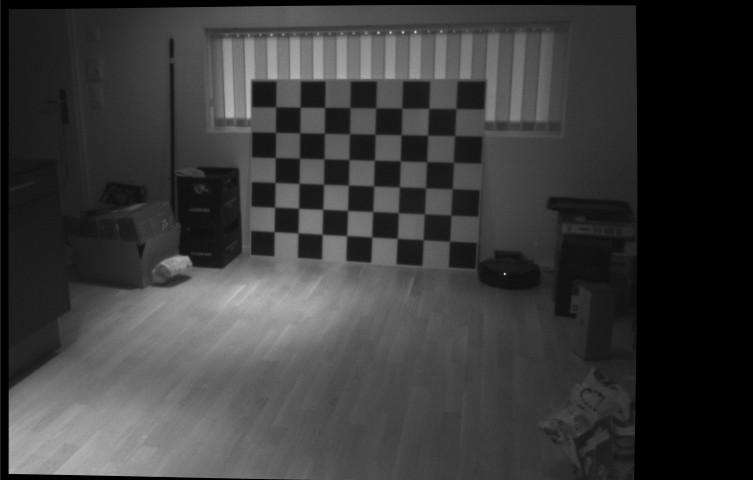
\includegraphics[width=0.4\textwidth]{img/calib0_left_rect.jpg}}
	\subfloat[right image after rectification]{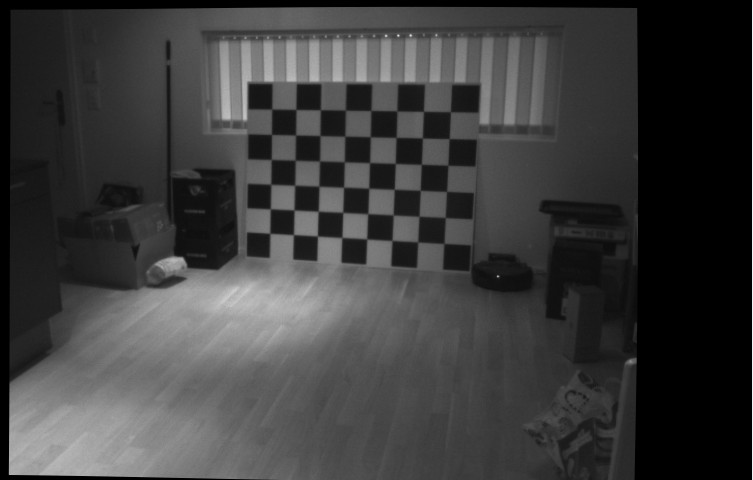
\includegraphics[width=0.4\textwidth]{img/calib0_right_rect.jpg}}
	\caption{Top: Two images used to calibrate the camera, Bottom: New images after rectify}\label{fig:calibration_real}
\end{figure}

Figure \ref{fig:calibration_real} shows a ``real'' example of a calibrated stereo camera. In comparison to example \ref{fig:stereo_calib} this calibration also corrects distortion and equalizes fx and fy for both cameras.\\

Another thing Stereo Calibration can calculate is the baseline of the two cameras. The baseline is the distance of the centers of the left and the right camera. For that we have to specify the length of one checkerboard field. With knowing that we can calculate the baseline. However, the calibration process will output focal length in pixels times baseline in meters as shown in equation \ref{eq:bf}. As we will see in equation \ref{eq:depth} this is the value needed for calculating the depth from disparity.

\begin{equation}\label{eq:bf}
	b_f=\frac{b*f}{p_s}
\end{equation}

\begin{align*}
	b_f &:	\text{Output of calibration process}\\
	b &:		\text{basline in m}\\
	f &:		\text{focal lenght in m}\\
	p_s &:	\text{Pixel size in m}\\
\end{align*}

\section{Checkerboard Size}

For camera calibration it is important to use a big checkerboard. The bigger the better the calibration results get. The reason is hidden in equation \ref{eq:cm}. When we try to find the projection matrix we will always have a small error. This error comes from restrictions regarding resolution and misplacement while detecting corners. However, if the checkerboard is far away the error will be divided trough the distance because we are not interested in scale while doing camera calibration. This means the farer away the checkerboard is the smaller will be the influence of our error.\\
For calibrating the camera we can for example print a checkerboard on to an advertisement board as e.g. offered by \cite{mydisplay}.\\
To see how well the calibration process performed we have to analyze the reprojection error that can be received by stereoCalibExtended of OpenCV. The error should be below 0.5 pixels, the smaller the better.

\section{Econ Tara calibration}
For calibrating the Econ Tara camera we can use the econ\_calibration\_images.py scripts. It should be called as follows:
\begin{lstlisting}[language=bash]
python3 econ_calibration_images.py <calib folder> --size <checkerboard filed size>
\end{lstlisting}

The images in the folder <calib folder> are gray scale and have the form <name><counter>\_left and <name><counter>\_right. We can use the script extract\_channels.py to create the images:
\begin{lstlisting}[language=bash]
python3 extract_channels.py <camera> <hidraw> <calib folder>
\end{lstlisting}
This script expects the path to the Econ Tara camera, the path to the hidraw device (to set exposure) and the output folder.

\chapter{ORB SLAM}\label{chap:implementation}

In this chapter we discuss more deeply how ORB SLAM works and how we port it to the iMX8 processor.

\section{How it works}
ORB SLAM tries to find corners with the FAST corner detection. This gives us points which should lay on the intersection between two edges. We call this points keypoints. At the corners we later calculate the ORB descriptors which describes the keypoint.\\
If we have a stereo image we can search for the keypoints on both images and from that calculate the depth of each point. For this we need to do the steps shown in figure \ref{fig:orb_slam2}.

\begin{figure}[H]
  \begin{center}
		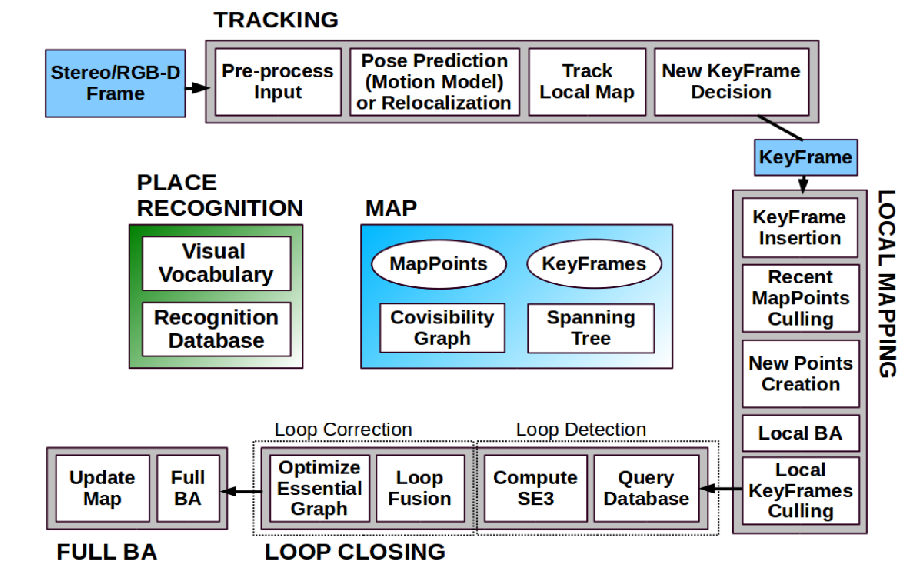
\includegraphics[width=0.9\textwidth]{img/orb_slam2.png}
  \end{center}
	\caption{ORB SLAM2 \cite{orbslam2}}\label{fig:orb_slam2}
\end{figure}

ORB SLAM uses multiple threads to improve the performance of the algorithm, this threads are described in the following sections.

\subsection{Tracking}

Tracking is the most important task where the algorithm tries to estimated the pose of the current image.
\begin{enumerate}
	\item Match descriptors from the left and the right image
	\item Calculate the difference in pixels between the keypoint on the left and on the right image
	\item Calculate the depth of the keypoint with formula shown in equation \ref{eq:depth}
	\item With known depth calculate the point position with camera as reference
	\item Match point descriptors with point descriptors from keyframe
	\item Estimate new camera pose with triangulation and RANSAC
	\item Check if this frame is a potential keyframe.
\end{enumerate}
The potential keyframe check is done by checking how many frames were captured since the last keyframe, if a lot of outliers were detected and if more than 35\% of points are new with regards to the reference keyframe.\\

\subsection{Local Mapping}
Local mapping tries to map the newly found keypoints into the world map.
\begin{enumerate}
	\item Transform the new keypoints to the global coordinate system based on the camera pose
	\item Do a bundle adjustment. It is likely that points we already know do not 100\% match the position where we see the points. Bundle adjustment fuses the position of points seen more than once.
	\item Check if more than 10\% of the points in the current frame compared to the points in all keyframes are new. If not we drop the keyframe for future use.
\end{enumerate}

\subsection{Loop Closing}
Loop closing tries to detect loops and will then do a bundle adjustment to increase the precision of the point cloud.
\begin{enumerate}
	\item Match latest keyframe with all keyframes stored in the database with DBoW2 \cite{dbow}
	\item Optimize correspondent point by doing bundle adjustment over key frame poses and point location
\end{enumerate}

\begin{equation}\label{eq:depth}
	d=\frac{f*b}{p_s*\Delta}\\
	\Delta=u_{left}-u_{right}
\end{equation}
\begin{align*}
	d &:					\text{depth}\\
	b &:					\text{baseline in m}\\
	f &:					\text{Focal length in m}\\
	p_s	&:				\text{Pixel size in m}\\
	\Delta &:			\text{Difference between x position on left and rigth image in pixels}\\
	\u_{left} &:	\text{X Position of keypoint on left image}\\
	\u_{right} &: \text{X Position of keypoint on right image}
\end{align*}

\begin{equation}\label{eq:orb_pos}
	y=\frac{d*u}{f_u}\\
	x=\frac{d*v}{f_v}
\end{equation}
\begin{align*}
	y &:				\text{Y position with camera 0}\\
	x &: 				\text{X position with camera 0}\\
	d &: 				\text{Depth=Z position with camera 0}\\
	u,v &:			\text{X,Y position on image}\\
	f_u,f_v &:	\text{Focal length}
\end{align*}

\section{Comparison Mono to Stereo}\label{sec:monster}

In this work we only talk about stereo SLAM. But what are the differences to a monocular SLAM system?\\
A monocular camera can't see depth. This means that from one single image we can't estimate the keypoints in the 3D world. This means we need some kind of initialization process that will try to estimate the depth over several images. There are different strategies for solving the initialization problem. ORB SLAM calculates two models in parallel one if most points are laying on a plane and one model if most points are random distributed. In one model the Essential Matrix (Fundamental Matrix with only 5DoF) is searched while in the other model the homography matrix is searched. If the initialization succeeds one of this matrices will converge to a small reprojection error while the other wont. The new camera pose can be estimated by decomposing the converged matrix. Other approaches use a EKF and try to optimize the camera pose over the first n frames. The EKF starts with random depth values and converges after several frames to the ``real'' depth values.  For a monocular camera it is not possible to find all 6 DoF because the fundamental and homography matrix only have 5DoF. They therefore set the 6 parameter to 1 which means we don't get a real ``scale'' value. All measurements with only monocular cameras are therefore scales.

\section{Port to iMX8}\label{sec:orbport}

The iMX8 BSP is built with Yocto. NXP and Toradex provide a BSP layer which contains a kernel and all necessary proprietary libraries for OpenGL. OpenCV is already part of the image fsl-image-qt5. How we build the BSP and the SDK is out of scope of this project. Please check the following references:\\
\begin{itemize}
	\item Yocto project \cite{yocto}
	\item Toradex BSP \cite{toradex_bsp}
\end{itemize}

From the Yocto build we can also receive an SDK which contains a ARM64 toolchain that can be used to compile additional programs and libraries. This toolchain was used to build the ORB SLAM2 for the iMX8. For the following section we assume that the toolchain is installed under/opt/fsl-imx-x11/4.9.51-mx8-beta

\subsection{Pangolin}
Pangolin \cite{pangolin} is required by ORB SLAM for showing the sparse map and the camera pose. A simple git checkout of the pangolin sources is enough to receive the sources. Before building the project with CMake the following patch should be applied:
\begin{lstlisting}
diff --git a/CMakeLists.txt b/CMakeLists.txt
index 32a2d78..683ef38 100644
--- a/CMakeLists.txt
+++ b/CMakeLists.txt
@@ -15,6 +15,9 @@ SET(CPACK_DEBIAN_PACKAGE_MAINTAINER "Steven Lovegrove")
 SET(CPACK_PACKAGE_VERSION_MAJOR ${PANGOLIN_VERSION_MAJOR})
 SET(CPACK_PACKAGE_VERSION_MINOR ${PANGOLIN_VERSION_MINOR})
 SET(CPACK_PACKAGE_VERSION_PATCH "0")
+SET(CMAKE_INCLUDE_SYSTEM_FLAG_CXX "-I")
+SET(CMAKE_INCLUDE_SYSTEM_FLAG_C "-I")
+
 include(CPack)
 
 option( BUILD_EXAMPLES "Build Examples" ON )
\end{lstlisting}

After that the following commands should be done:
\begin{lstlisting}[language=bash]
. /opt/fsl-imx-x11/4.9.51-mx8-beta/environment-setup-aarch64-poky-linux
mkdir build
cd build
cmake -DCMAKE_INSTALL_PREFIX=<INSTALL_DIR> ..
make -j
make install
\end{lstlisting}

This will build the Pangolin library for ARM64. INSTALL\_DIR should point to a directory which can be used as local ``root filesystem''. This root filesystem can later be copied via scp to the iMX8.

\subsection{OpenCV}\label{sec:opencv}
To get the modified ORB SLAM 2 working the OpenCV version from \cite{opencv_se} should be used. The branch se-3.4.3 contains some a modifications that allows us to reuse the image pyramid generated by ORB. Also the CMake flags are changed to allow compilation on iMX8. Additionally we need to compile OpenCV Contribute \cite{opencv_contrib} sources version tag 3.4.3. To build OpenCV the following commands are required:
\begin{lstlisting}[language=bash]
. /opt/fsl-imx-x11/4.9.51-mx8-beta/environment-setup-aarch64-poky-linux
. /opt/fsl-imx-x11/4.9.51-mx8-beta/sysroots/x86_64-pokysdk-linux/environment-setup.d/cmake.sh

mkdir build
cd build

export PKG_CONFIG_LIBDIR=/opt/fsl-imx-x11/4.9.51-mx8-beta/sysroots/aarch64-poky-linux/usr/lib/pkgconfig/
cmake -DWITH_ITT=NO -DWITH_LIBV4L=YES -DWITH_TBB=NO -DOPENCV_EXTRA_MODULES_PATH=<path to OpenCV contrib> -DCMAKE_BUILD_TYPE=Release ..
\end{lstlisting}

The libraries found in the lib directory can the be copied to /usr/lib on the iMX8.

\subsection{ORB SLAM 2}
We use the sources of ORB SLAM 2 \cite{orbslam2_impl}. Instead of using the sources from ORB SLAM directly the modified sources \cite{orbslam2_se} under branch iMX8 should be used. It contains some fixes for newer compiler versions as well as additional sources for the ECON Tara camera. After checking out the sources the following commands should build the binaries:\\
\begin{lstlisting}[language=bash]
. /opt/fsl-imx-x11/4.9.51-mx8-beta/environment-setup-aarch64-poky-linux
mkdir build
cd build
cmake -DPangolin_DIR=<INSTALL_DIR/usr/lib/cmake/Pangolin> -DCMAKE_INSTALL_PREFIX=<INSTALL_DIR> -DOpenCV_DIR:PATH=<OPENCV_BUILD_DIR> ..
make -j
make install
\end{lstlisting}

This will build ORB SLAM for ARM64. INSTALL\_DIR is the same directory as it was for Pangolin. After that we can copy the whole INSTALL\_DIR to the iMX8 root directory and start econ\_stereo for starting the SLAM system. The OPENCV\_BUILD\_DIR should point to the build directory of OpenCV in section \ref{sec:opencv}.

\subsection{ORB SLAM 2 usage}

For the Econ Tara a special stere\_econ application is available. This application can be called as follows:
\begin{lstlisting}[language=bash]
./stereo_econ path_to_vocabulary path_to_settings path_to_video
\end{lstlisting}

The first argument path\_to\_vocabulary is the ORB dictionary for DBoW2, path\_to\_settings should point to the Econ.yaml and path\_to\_video points to the Econ Stereo Camera device.\\
In comparison to the orignal ORB SLAM 2 implementation some additional parameters are added:\\
\begin{tabular}{l l}
stereosgbm.cn & CN parameter fo sgbm \\
stereosgbm.preFilterCap & Pre filter capacity for sgbm \\
stereosgbm.windowSize & Window size for sgbm \\
stereosgbm.blockSize & Block size for sgbm \\
stereosgbm.minDisparity & Minimum disparity for sgbm \\
stereosgbm.speckleRange &  Speckle Range for sgbm \\
stereosgbm.disp12MaxDiff & Max diff for sgbm \\
stereosgbm.uniquenessRatio & Uniqueness ratio for sgbm \\
stereosgbm.speckleWindowSize & Speckle window size for sgbm \\
stereosgbm.numberOfDisparities & Total number of disparities for sgbm \\
cpu.system & CPU assigned to system thread \\
cpu.stereoleft & CPU assigned to orb thread for left image \\
cpu.stereoright & CPU assigned to orb thread for right image \\
cpu.loopclosing & CPU assigned to loop closing thread \\
cpu.localmapping & CPU assigned to local mapping thread \\
cpu.densify & CPU assigned to densify thread \\
cpu.viewer & CPU assigned to viewer \\
Densify.enabled & 0 if densify is disabled 1 if enabled \\
ORBextractor.orbextractor & Orb extractor: 0->Original, 1->OpenCV, 2->OpenCV OCL \\
Densify.topmargin & top margin for depth image \\
Densify.bottommargin & bottom margin for depth image \\
Densify.leftmargin & left margin for depth image \\
Densify.rightmargin & right margin for depth image \\
\end{tabular}\\

The SGBM features are hard to tune the values in Econ.yaml were taken from the stereo\_match.cpp example of OpenCV \cite{opencv_se}. The ORBextractor.orbextractor can be used to switch between different ORB implementations in section \ref{sec:results}.

\chapter{Densification}

\begin{figure}[H]
  \begin{center}
		\includegraphics[width=0.9\textwidth]{img/dense_cloud.png}
  \end{center}
	\caption{A dense cloud generated with SGBM and ORB SLAM}\label{fig:dense_cloud}
\end{figure}

ORB SLAM only delivers a very sparse map. Therefore, it can't be used e.g. for creating a map or to reconstruct 3D objects. It's focus lays on delivering a stable pose of camera rather than on creating a useful map of it's environment. In this section we discuss how we can improve ORB SLAM by densifing the point cloud as shown in figure \ref{fig:dense_cloud}. We also show a ruff implementation which however isn't state of the art as we will see later.\\
In the first section we will see how the stereo images can be used to create a depth map. The next section describes how to use the depth map to generate a point cloud. The two last sections discusses two possibilities how a depth map of several poses could be fused together. However, as we will see the current approach doesn't work as expected because the point cloud increases too fast and the algorithms slows down massively.

\section{Depth Map}

A depth map is an image that contains depth values instead of color intensities. They are normally generated from stereo cameras or from ToF cameras. We will only talk about how depth images are generated from stereo cameras. Image \ref{fig:depth} shows such an image that was generated from the images of a stereo camera.

\begin{figure}[H]
	\centering
	\subfloat[left image]{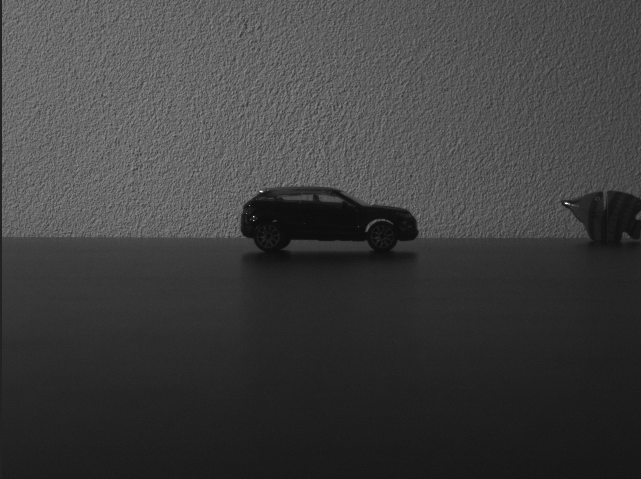
\includegraphics[height=100px]{img/disparity_left.png}}
	\subfloat[right image]{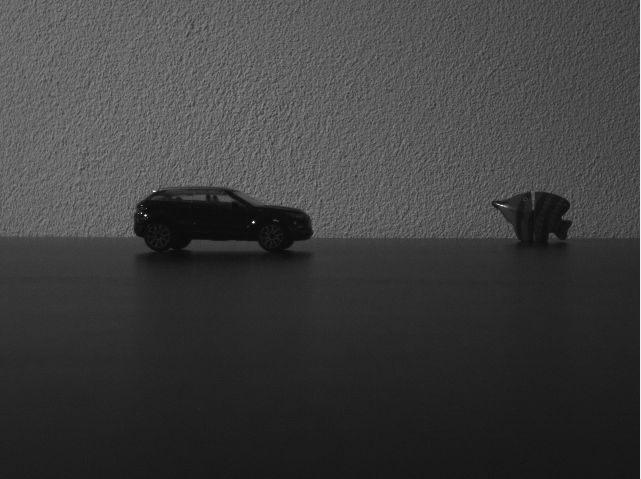
\includegraphics[height=100px]{img/disparity_right.png}}
	\subfloat[depth image]{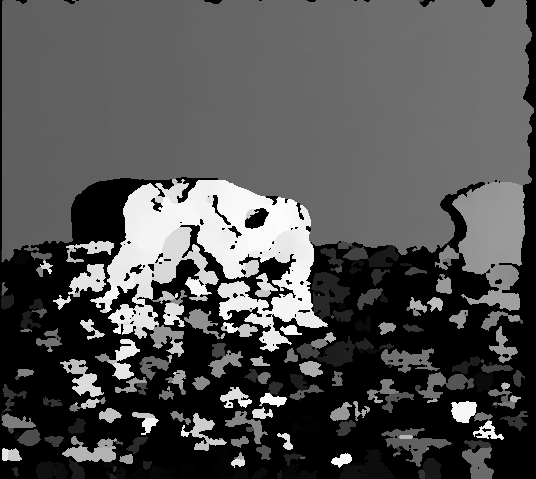
\includegraphics[height=100px]{img/disparity.png}}
	\caption{Depth image from stereo}\label{fig:depth}
\end{figure}

As we can see in figure \ref{fig:depth} the depth image is noisy in areas where the we have low or no texture. This is due to how the algorithm works. The algorithm does an intensity block matching. Because the camera is aligned horizontally the algorithm begins matching at the pixel position of the left image and matches from there to the right as shown in figure \ref{fig:disparity}. The horizontal line is also called epipolar line. The distance of a point on the left image to the right image is called disparity. An object which is farer away will have less disparity than an object which is near. A point at infinity will have a disparity of zero.

\begin{figure}[H]
  \begin{center}
		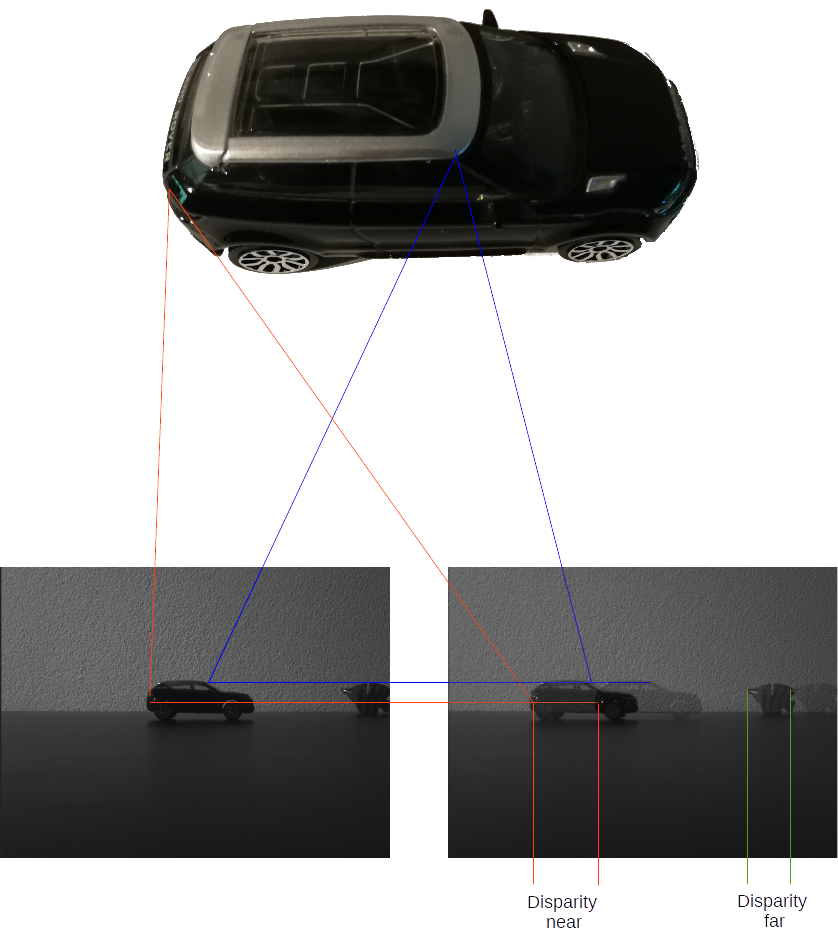
\includegraphics[width=0.9\textwidth]{img/disparity_concept.png}
  \end{center}
	\caption{Disparity with epipolar (horizontal) line, left: left image, right: right image with transparent left image}\label{fig:disparity}
\end{figure}

We use a Block Matching algorithm which matches for each pixel a template from the left image with the right image. The pixel with the lowest value is taken as best match and the offset is the disparity. However this algorithm is prone to noise therefore a modified version of this algorithm is used called Semi Global Block Matching (SGBM) \cite{sgbm}. In comparison to normal Block Matching this algorithm penalties if neighbour pixels have a big disparity difference. We additionally calculate the disparity for the left and right image so that we also get values for pixels that are only visible in one image. Further we can generate a confidence map if pixels have different disparities when we do left and right matching.

\section{Point Cloud from Depth}

From the Depth map generated by the previous section we can then calculate a dense point cloud based on the current pose. We transform the depth information into the three dimensional space. An example of such a point cloud can be seen in figure \ref{fig:pointcloud}. The point cloud is generated from the depth image by transforming each pixel with the current camera pose.

\begin{equation}\label{eq:point_cloud_depth}
	\begin{pmatrix}
			X \\
			Y \\
			Z
	\end{pmatrix}=
	\begin{pmatrix}
		r_{00} & r_{01} & r_{02} & t_x \\
		r_{10} & r_{11} & r_{12} & t_y \\
		r_{20} & r_{21} & r_{22} & t_z \\
	\end{pmatrix}*
	\begin{pmatrix}
		x,
		y,
		d,
		1
	\end{pmatrix}
\end{equation}
\begin{align*}
	X,Y,Z &:			\text{World position of the pixel}\\
	r_{ij} &:			\text{Rotation elements of pose}\\
	t_{x,y,z} &:	\text{Translation elements of pose}\\
	x,y:					\text{u,v translated to world, see \ref{eq:orb_pos}}\\
	d &:					\text{depth}
\end{align*}

\begin{figure}[H]
  \begin{center}
		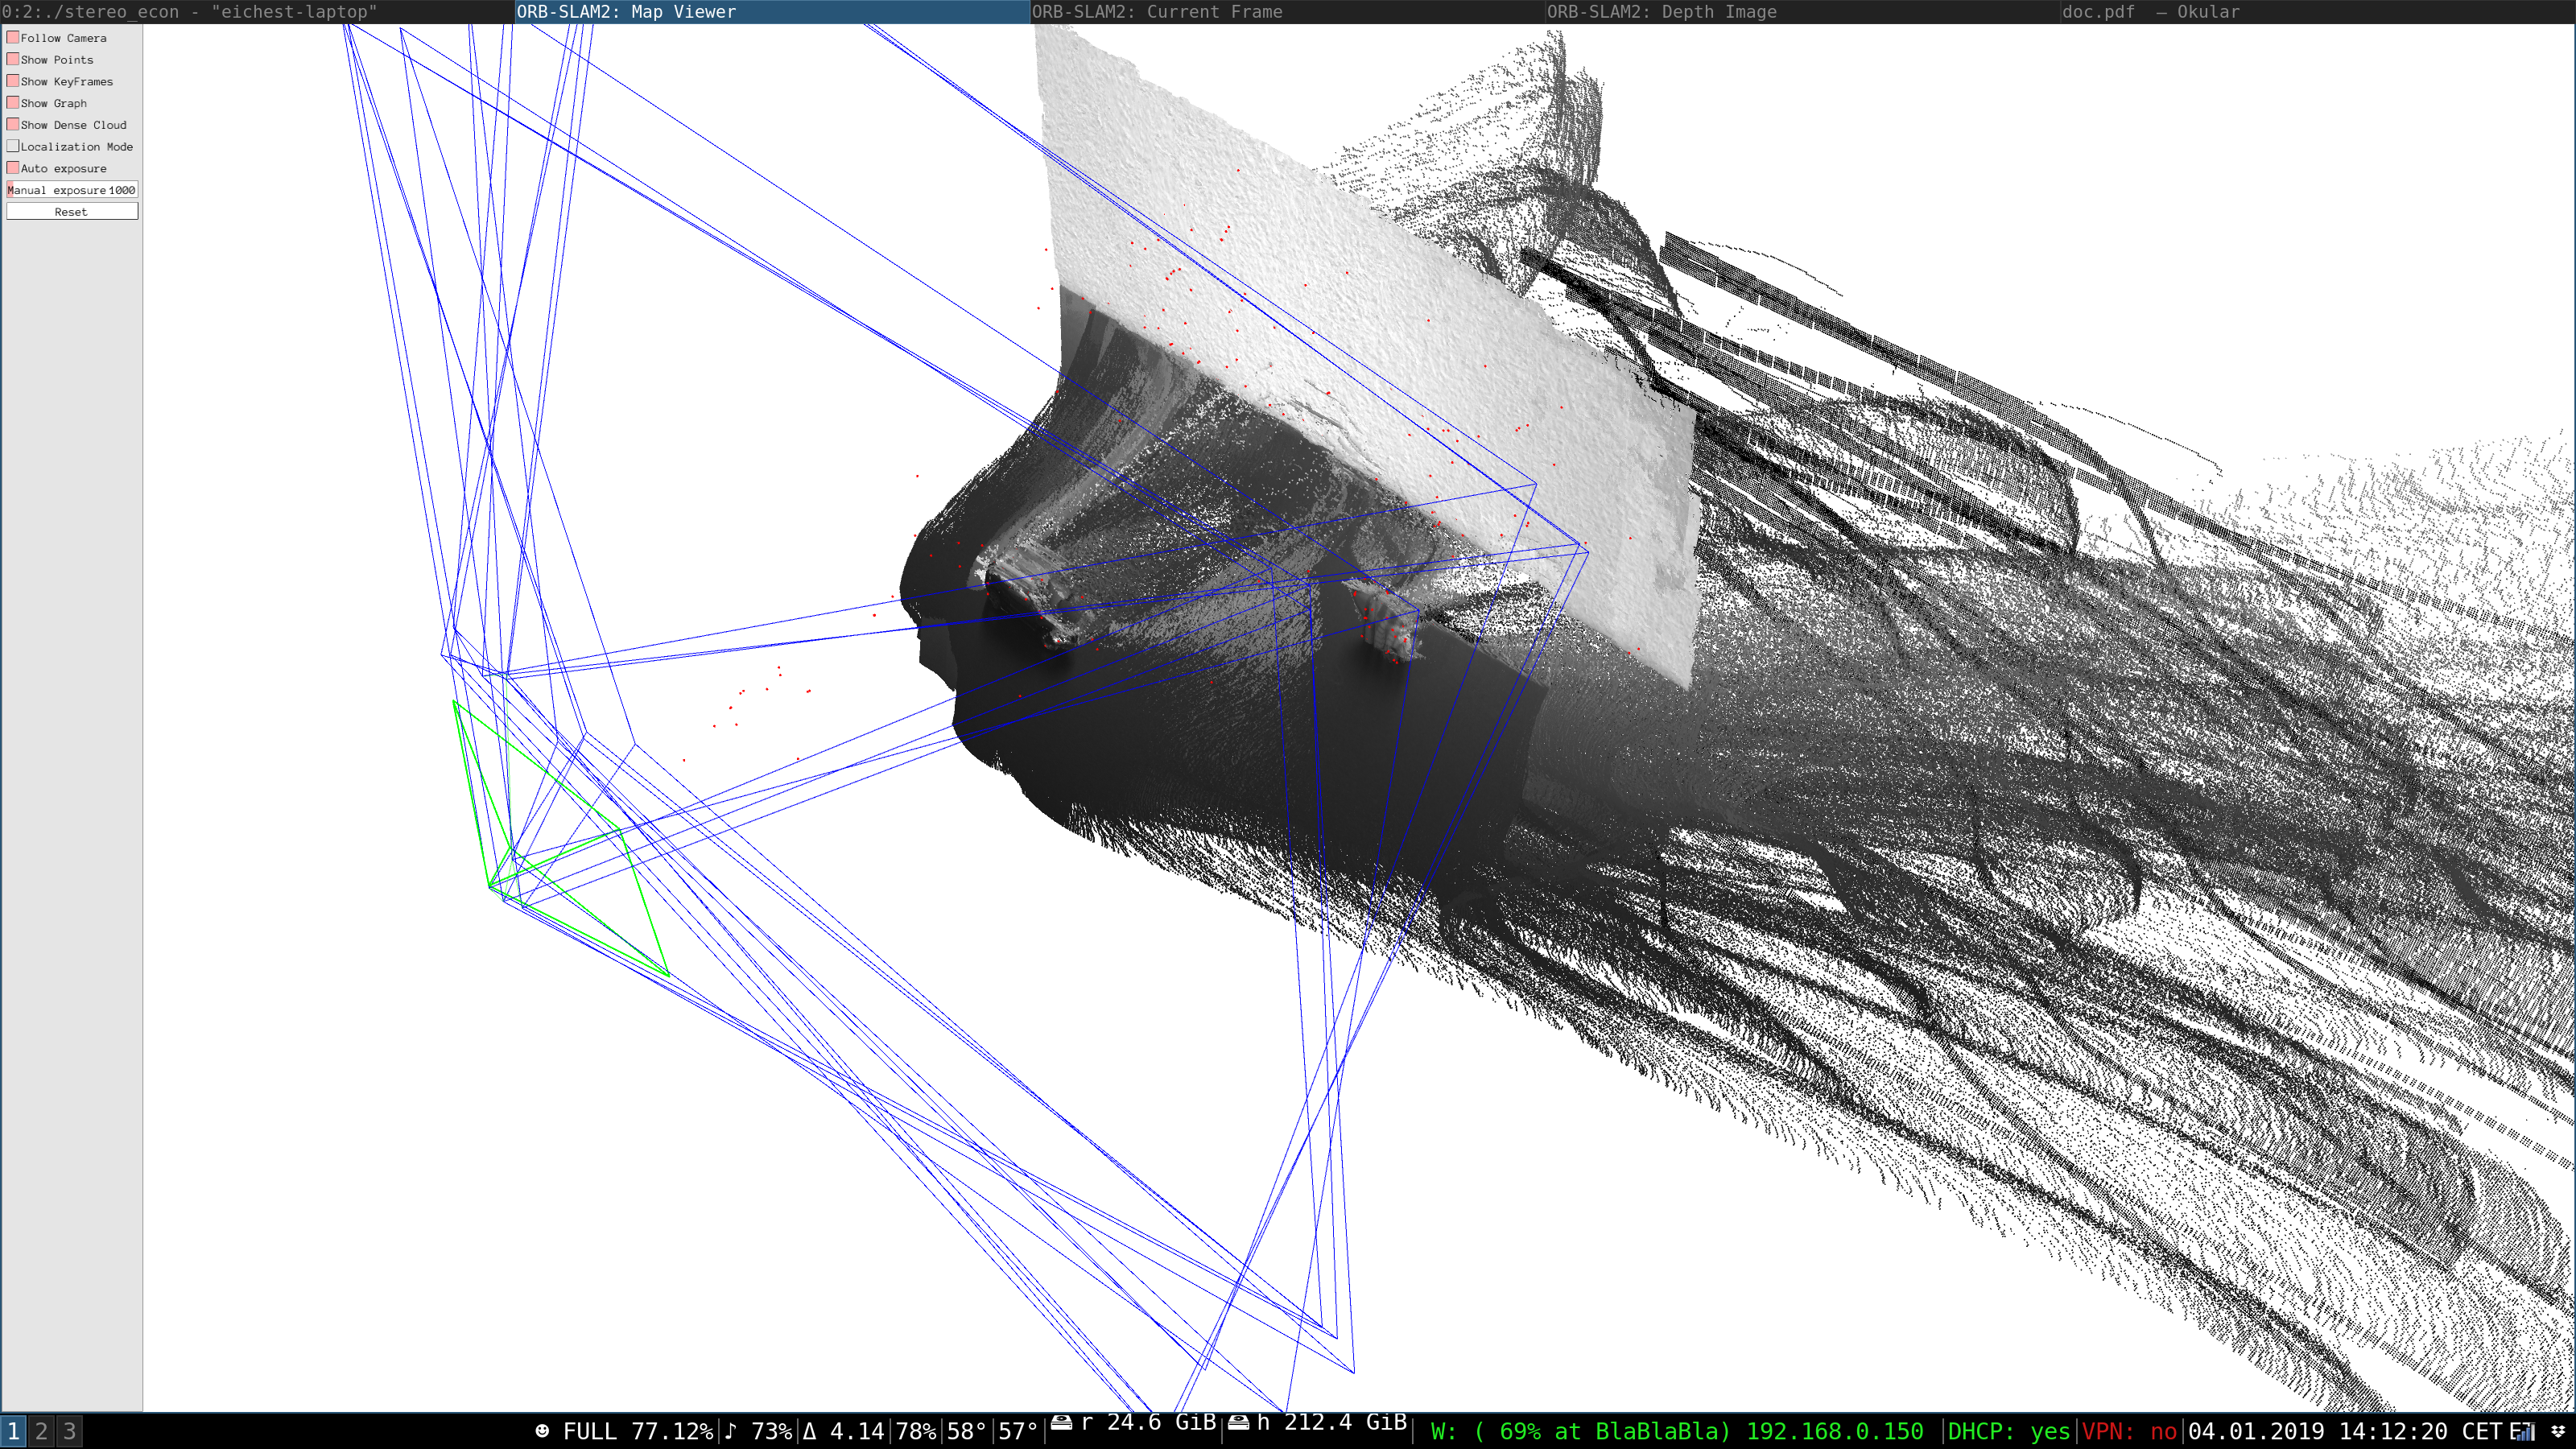
\includegraphics[width=0.9\textwidth]{img/pointcloud.png}
  \end{center}
	\caption{Dense point cloud generated from different key frames}\label{fig:pointcloud}
\end{figure}

To reduce the CPU load we only add new dense points to the cloud for keyframes. What we can see in figure \ref{fig:pointcloud} is that because of the uncertainty of the depth map we have tons of outliers. Further we don't fuse points at the same location therefore we generate a lot of points that have the same position within a statistic probability.

\section{Point Cloud fusion}

There are different papers that describe the problem of point cloud fusion. If you have two views that partially show the same region you will always have to merge the overlapping part. Here I would like to shortly point out two possibilities for that. REMODE and Volumetric 3D Mapping.

\subsection{REMODE}

REMODE uses a probabilistic approach to fuse data from different views. Only points that have a high enough probability for being there are actually drawn on the 3D map. This generates a semi dens point cloud which has a high probability of being true. However it requires a lot of frames seeing the same scene for getting high accuracy, this is exactly what we try to avoid because we already have problems to perform well with our current approach. Therefore this algorithm can't be used in embedded systems for our dense cloud.

\subsection{Volumetric 3D Mapping}

The approach of using a volumetric 3D mapping is quite interesting. The algorithm is designed to run on a CPU only. It assigns a box to each 3D pixel and grids this boxes in an octree. If a new pixel should entered the algorithm check whether it would fix in an existing box. Unfortunately, a short test implementation showed that also this approach would use too much CPU power. Therefore, we have to think about a different approach.

\chapter{Discussion}

In this chapter we discuss the current status of this work. We analyse the achievements and see if we can improve the approach to achieve realtime location and mapping.

\section{Results}\label{sec:results}

The current implementation is heavily based on the original ORB SLAM2 implementation as described in section \ref{sec:orbport}. Because we used normal ORB SLAM the results from the original paper are still valid. However, what we are interested in is the realtime frame rate and the therefore the time used per frame. The original ORB SLAM2 implementation calculates exactly this time per frame and writes out the mean and median time after each run. For comparison we used the KITTI04 dataset with 271 images. The resolution of each image is 1226x370 where the ECON Tara has a resolution of 752x480. The KITTI dataset is a standard benchmark for SLAM therefore this one was taken. In comparison to Euroc another dataset it has smaller sequences and finishes therefore faster.\\\

We compare the ORB SLAM ORB implementation with the ORB implementation from OpenCV. To be fair we reduce the feature count from 1000 to 800 because OpenCV ORB normally finds more features than the ORB SLAM implementation. The bigger the point cloud gets the slower the algorithm performs, therefore it wouldn't be a fair comparison.

median tracking time: 0.358698
mean tracking time: 0.362126


\begin{table}
	\begin{tabular}{  | l | l | l | l | l | l | }
		\hline
		\textbf{CPU} & \textbf{Impl.} & \textbf{feat.} & \textbf{feat. det.} & \textbf{median tt} & \textbf{mean tt} \\ \hline
		iMX8 & ORB & 1000 &  548 & 0.18307 & 0.185202 \\ \hline
		iMX8 & ORB, Linux scheduled & 1000 & 548 & 0.390867 & 0.387753 \\ \hline
		iMX8 & OpenCV & 1000 & 757 & 0.190571 & 0.210072 \\ \hline
		iMX8 & OpenCV & 800 & 610 & \textbf{0.155441} & \textbf{0.167176} \\ \hline
		iMX8 & OpenCV, Linux scheduled & 800 & 610 & 0.358689 & 0.362126 \\ \hline
		iMX8 & OpenCV OpenCL & 800 & 610 & 0.50622 & 0.771859 \\ \hline
		i5-7Y54 & ORB & 1000 & 546 & 0.18884 & 0.184628 \\ \hline
		i5-7Y54 & OpenCV & 1000 & 756 & 0.154901 & 0.152786 \\ \hline
		i5-7Y54 & OpenCV & 800 & 610 & 0.135715 & 0.132304 \\ \hline
	\end{tabular}
	\caption{Comparison of ORB SLAM tracking time in KITTI04 using ORB or OpenCV implementation}
  \label{tab:result}
\end{table}

As we can see from table \ref{tab:result} we can achieve the best timings on the iMX8 when using the OpenCV ORB SLAM implementation. We could extend this version so that it behaves the same as the ORB SLAM implementation and would still benefit from the improvement. However, we are still at a very low frame rate of around 6 frames per seconds. When we compare this result to a i5-7Y54 x86 processor we are not far away where we get around 7fps. Unfortunately none of this results is near to realtime it works well for slow movements but it can't handle fast movements because of the bad performance. The biggest disappointment is that the OpenCL implementation of ORB in OpenCV is worse than the CPU implementation. We can't therefore increase the performance by using the GPU instead of the CPU. Even if we would tweak the OpenCL implementation we probably wouldn't get close to the CPU version.

\section{Optimizations}

The current frame rate on the target as well as on a laptop with slow CPU is too low. This makes it difficult to get a robust mapping in realtime.

\subsection{Different ORB Implementation}
By replacing the ORB algorithm from ORB SLAM with the one from OpenCV we can see that higher framerates are possible. However, this improves it only by around 20\% and we don't provide from the better distribution of ORB SLAM. This could of course be added to OpenCV ORB by modifying the sources.

\subsection{Using OpenCL}
OpenCV ORB also supports the finding of FAST corners and ORB descriptor calculation with OpenCL. However, a first test showed that using OpenCL is even slower than using the CPU. The reason for this is probably that the overhead is too high. It could be that an algorithm that is designed to run completely on GPU would benefit a lot more.

\subsection{Reduce Resolution}
Using lower resolution images would improve the performance of the algorithm. However, this is not something we want to do because it also decreases the stability in the end. With a resolution of 752x480 we already limit the resolution to a realistic level for embedded devices.

\section{Problems}

\subsection{Big Algorithm}
ORB SLAM is a powerful algorithm. It is also quite complicated in how it works. Bundle adjustment seems to be one of the most powerful optimization technics to improve the accuracy of SLAM. However, it is also not supper performance.

\subsection{Descriptor Calculation}
ORB descriptors are also very stable over different images and can even handle different illumination up to certain level. However, it seems that calculating the descriptors consumes quite some CPU power.

\subsection{Lot of dependencies}
It is clear how the algorithm works, however the implementation is quite complicated. It uses two additional libraries to OpenCV g2o and libeigen, g2o is even modified. This makes it hard to find a entry point for optimization.

\subsection{Entrypoint}
Even when only trying to optimize the tracking thread we are somehow dependent on local mapping because we need the point cloud. So it's also hard to find an entry point for optimization here.\\

\subsection{Newer approaches}
A lot of newer approaches for SLAM nowadays talk about direct approaches. It seems that the overhead of direct box matching can sometimes be less problematic than to calculate descriptors. If high frame rates can be achieved the search radius is very limited which reduces the CPU cost even more. By using IMU to track the movement we could probably limit the search radius even more which speeds up the direct approaches even more. This is unfortunately not true for ORB SLAM because we always have to do the heavy calculation of ORB descriptors. Therefore the next chapter should give a brief overview of what approach we should investigate in the future.

\chapter{Direct Approach}

Because a lot of newer papers describe sparse direct approaches as faster than indirect methods we will analyze one of them here. This could be the basis for further work specially when using it together with data from the IMU.

\section{SVO}

SVO stands for sparse visual odemetery. It is a sparse direct approach to the SLAM problem. The first monocular implementation was released as open source however the improved SVO2 source code is not publicly available. However, the paper describes the algorithm in good enough detail so that it should be possible to do a similar implementation. The algorithm is ruffly constructed as follows.

Initialization (Stereo):
\begin{enumerate}
	\item Search corner points with FAST
	\item Split the image into areas of fixed size (e.g. 32x32)
	\item Take the FAST corner with maximum response in each area if there is any
	\item (optional) If there is no FAST corner take the point with highest gradient on an edge (see \ref{fig:svo})
	\item With a stereo camera we can do a template matching for each of this ~100 points to find the depth of each point
	\item Add current frame as key frame
\end{enumerate}

Tracking:
\begin{enumerate}
	\item For each point we try to minimize the photometric error (intensity difference)
		\subitem (optional) The motion model could be improved via IMU
	\item By using Levenberg-Marquardt we find the best transformation matrix that describes our movement
	\item (optional) For each point we calculate the backprojection and calculate packprojection into the image
	\item (optional) From the backprojection we calculate the error between where we see the point and where it probably is
	\item (optional) We adjust the 3D points with bundle adjustment to minimize the backprojection error of the key frame and the new image
\end{enumerate}

\begin{figure}[H]
  \begin{center}
		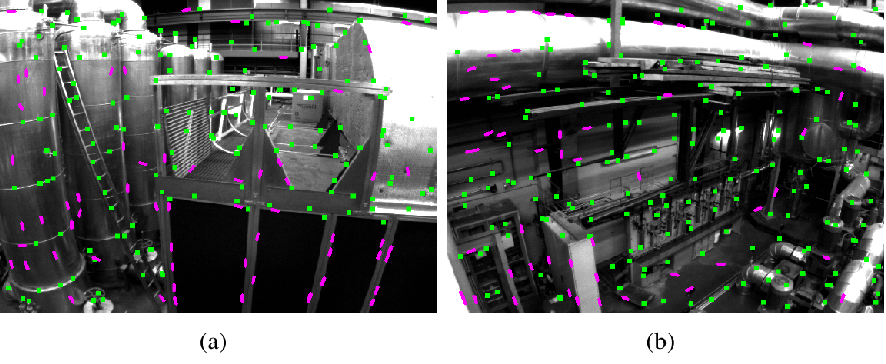
\includegraphics[width=1.0\textwidth]{img/svo.png}
  \end{center}
	\caption{Example of sparse points used by SVO in Euroc dataset \cite{svo}. The green points are fast corners the magenta points are edgelets used in areas with no corners}\label{fig:svo}
\end{figure}

This algorithm can't do loop closing as ORB SLAM does. However, it would be possible to add such improvement if necessary (e.g. by using orb descriptors only on reference frames). Due to it's simplicity they report 13.27ms to process one 640x480 frame in EUROC Machine Hall 1 on an Nvidia Jetson TX1. The CPU of this processor is comparable to the one on the iMX8. This would end up in a frame rate of up to 75fps which is above 60fps what is the maximum of the Econ camera. They also split the algorithm into two threads, therefore even higher framerates could be achieved on a multiprocessor system.

\section{Densification}

In the SVO paper they describe the possibility to do densification based on the sparse points. The problem however is that dense clouds can consume a lot of graphics memory, which is not something you have granted on embedded systems. Because SVO is using corners as key points an approach could be that a mesh is created between all this points. To get a better feeling of the environment the keyframes can be used as textures so a dense mesh with a sparse point cloud can be created. To increase the resolution we simply need to get closer to the object, because in this case more corners are detected which means the map get denser. This would be computationally less expensive further the complicated fusion of point clouds is easier and could event be avoided by simply throwing away points with less resolution taken from a view farer away. We can argue that the same approach could be used for ORB SLAM however, the problem there is that we can't use any corner but only corners with good ORB responses. Therefore not all corners can be used which means the mesh will be less precise, maybe even hides important details.

\section{Outlook}
SVO SLAM is espacialy interesting because of it's simplicity and because it is possible to remove a lot of optional features. By removing this optional features the tracking results are getting worse but if we combine tracking with data from the IMU we can hopefully compensate the loss of precision. Together with a stereo camera we also don't need the complicated initialization process described in the SVO paper, because we can directly calculate the depth of each point with the first frame.

\chapter{Conclusion}
Unfortunately the current results specially regarding realtime capabilities do not look promising for ORB SLAM. It is hard to optimize the algorithm because of its complexity. Event with multithreading and multiprocessing in place we still have dependencies between tracking and local mapping. Therefore we propose to use a direct sparse approach for doing SLAM instead of using an indirect sparse approach. The disadvantage of the computationally more expensive pose estimation has the advantage of not having the need of extracting expensive features. The whole algorithm also can be reduced to a simpler implementation when not using all optional features.

\listoffigures
 
\begin{thebibliography}{1}

	\bibitem{orb}
	E. Rublee, V. Rabaud, K. Konolige, and G. Bradski
	\textit{ORB: an efficient alternative to SIFT or SURF} 
	IEEE International Conference on Computer Vision (ICCV), Barcelona, Spain, November 2011, pp. 2564–2571.

  \bibitem{orbslam}
  Raul Mur-Artal, J. M. M. Montiel, Juan D. Tardos
  \textit{ORB-SLAM: a Versatile and Accurate Monocular SLAM System}
  arXiv:1502.00956v2

  \bibitem{orbslam2}
  Raul Mur-Artal, J. M. M. Montiel, Juan D. Tardos
  \textit{ORB-SLAM2: an Open-Source SLAM System for Monocular, Stereo and RGB-D Cameras}
	arXiv:1610.06475v2 

	\bibitem{dtam}
	Richard A. Newcombe, Steven J. Lovegrove and Andrew J. Davis
	\textit{DTAM: Dense Tracking and Mapping in Real-Time}
	doi:10.1109/ICCV.2011.6126513

	\bibitem{svo}
	Christian Forster et al.
	\textit{SVO: Semi-Direct Visual Odometry for Monocular and Multi-Camera Systems}
	doi:10.1109/TRO.2016.2623335

	\bibitem{fast}
	E. Rosten, R. Porter, and T. Drummond 
	\textit{Faster and better: A machine learning approach to corner detection}
	doi:10.1109/TPAMI.2008.275


	\bibitem{mydisplay}
	mydisplay.ch,
	\textit{Advertisement board manufacturer}
	https://www.mydisplays.ch/

	\bibitem{yocto}
	Yocto Project,
	\textit{Yocto Project Mega Manual}
	https://www.yoctoproject.org/docs/latest/mega-manual/mega-manual.html

	\bibitem{toradex_bsp}
	Toradex AG,
	\textit{Build Apalis iMX8 OpenEmbedded Project Bring-up Image}
	https://developer.toradex.com/software/linux/linux-software/build-apalis-imx8-yoctoopenembedded-bring-up-image

  \bibitem{orbslam2_impl}
  Raul Mur-Artal, J. M. M. Montiel, Juan D. Tardos
  \textit{ORB-SLAM2 Implemenation}
	https://github.com/raulmur/ORB\_SLAM2

  \bibitem{orbslam2_se}
  Raul Mur-Artal, J. M. M. Montiel, Juan D. Tardos
  \textit{ORB-SLAM2 Implemenation modified version}
	https://github.com/eichenberger/ORB\_SLAM2.git

	\bibitem{dbow}
	D. Gálvez-López and J. D. Tardós,
	\textit{Bags of binary words for fast place recognition in image sequences}
	IEEE Trans. Robot., vol. 28, no. 5, pp. 1188–1197, 2012.

	\bibitem{pangolin}
	Steven Love Grove,
	\textit{Pangolin Project}
	https://github.com/stevenlovegrove/Pangolin.git

	\bibitem{sgbm}
	Heiko Hirschmüller,
	\textit{ Stereo Processing by Semi-Global Matching and Mutual Information}
	IEEE TRANSACTIONS ON PATTERN ANALYSIS AND MACHINE INTELLIGENCE
	 
	\bibitem{rvc}
	Peter Corke,
	\textit{Robotics, Vision and Control}
	Springer, ISBN 978-3-319-54413-7, chapter 11+12, page 319+

	\bibitem{ransac}
	wikipedia,
	\textit{RANSAC}
	https://de.wikipedia.org/wiki/RANSAC-Algorithmus

	\bibitem{opencv_se}
	OpenCV,
	\textit{OpenCV computer vision framework (modified version)}
	https://github.com/eichenberger/opencv

	\bibitem{opencv_contrib}
	OpenCV,
	\textit{OpenCV computer vision framework extensions}
	https://github.com/opencv/opencv\_contrib

\end{thebibliography}


\end{document}
